\documentclass[a4paper,14pt]{extreport}
  \usepackage[left=1.5cm,right=1.5cm,
      top=1.5cm,bottom=2cm,bindingoffset=0cm]{geometry}
  \usepackage{scrextend}
  \usepackage[T1,T2A]{fontenc}
  \usepackage[utf8]{inputenc}
  \usepackage[english,russian,ukrainian]{babel}
  \usepackage{tabularx}
  \linespread{1.3}
  \usepackage[colorinlistoftodos]{todonotes}
  \usepackage{amssymb}
  \usepackage{color}
  \usepackage{amsmath}
  \usepackage{mathrsfs}
  \usepackage{listings}
  \usepackage{graphicx}
  \graphicspath{ {./images/} }
  \usepackage{lipsum}
  \usepackage{xcolor}
  \usepackage{hyperref}
  \usepackage{tcolorbox}

  \usepackage[framemethod=TikZ]{mdframed}
  \usepackage{wrapfig,boxedminipage,lipsum}
  \mdfdefinestyle{MyFrame}{%
  linecolor=blue,outerlinewidth=2pt,roundcorner=20pt,innertopmargin=\baselineskip,innerbottommargin=\baselineskip,innerrightmargin=20pt,innerleftmargin=20pt,backgroundcolor=gray!50!white}
   \usepackage{csvsimple}
   \usepackage{supertabular}
  \usepackage{pdflscape}
  \usepackage{fancyvrb}
  %\usepackage{comment}
  \usepackage{array,tabularx}
  \usepackage{colortbl}

  \usepackage{varwidth}
  \tcbuselibrary{skins}
  \usepackage{fancybox}
  \usepackage{spreadtab}


  \usepackage{tikz}
  \usepackage[framemethod=TikZ]{mdframed}
  \usepackage{xcolor}
  \usetikzlibrary{calc}
  \makeatletter
  \newlength{\mylength}
  \xdef\CircleFactor{1.1}
  \setlength\mylength{\dimexpr\f@size pt}
  \newsavebox{\mybox}
  \newcommand*\circled[2][draw=blue]{\savebox\mybox{\vbox{\vphantom{WL1/}#1}}\setlength\mylength{\dimexpr\CircleFactor\dimexpr\ht\mybox+\dp\mybox\relax\relax}\tikzset{mystyle/.style={circle,#1,minimum height={\mylength}}}
  \tikz[baseline=(char.base)]
  \node[mystyle] (char) {#2};}
  \makeatother
   % Цвета для гиперссылок
  \definecolor{linkcolor}{rgb}{0, 0.72, 0.92} % цвет ссылок
  \definecolor{urlcolor}{rgb}{0.0, 0.0, 1.0}% цвет гиперссылок
  \hypersetup{pdfstartview=FitH,  linkcolor=linkcolor,urlcolor=urlcolor,citecolor=red, colorlinks=true}

  \definecolor{ggreen}{rgb}{0.4,1,0}
  \definecolor{rred}{rgb}{1,0.1,0.1}
  \definecolor{amber}{rgb}{1.0, 0.75, 0.0}
  \definecolor{babyblue}{rgb}{0.54, 0.81, 0.94}
  \definecolor{amethyst}{rgb}{0.6, 0.4, 0.8}

  \usepackage{float}
  \usepackage{wrapfig}
  \usepackage{framed}
  %for nice Code{
  \lstdefinestyle{customc}{
    belowcaptionskip=1\baselineskip,
    breaklines=true,
    frame=L,
    xleftmargin=\parindent,
    language=C,
    showstringspaces=false,
    basicstyle=\small\ttfamily,
    keywordstyle=\bfseries\color{green!40!black},
    commentstyle=\itshape\color{purple!40!black},
    identifierstyle=\color{blue},
    stringstyle=\color{orange},
  }
  \lstset{escapechar=@,style=customc}
%}


\begin{document}
\renewcommand{\bibname}{Список використаної літератури}% -- переименуем название списка литературы


%указатель -- \cite{lit1}

\pagecolor{white}

%----------------------------------------1
\newtcbox{\xmybox}[1][red]{on line, arc=7pt,colback=#1!10!white,colframe=#1!50!black, before upper={\rule[-3pt]{0pt}{10pt}},boxrule=1pt, boxsep=0pt,left=6pt,right=6pt,top=2pt,bottom=2pt}

\begin{titlepage}
  \begin{center}
  \large
  Національний технічний університет України \\ "Київський політехнічний інститут імені Ігоря Сікорського"


  Факультет Електроніки

  Кафедра мікроелектроніки
  \vfill

  \textsc{РЕФЕРАТ}\\

  %{\Large Про виконання лабораторної роботи №1\\
  з дисципліни: «Фізико - технологічні основи наноелектроніки-2»\\[1cm]

  Реалізація кубитів для квантових комп'ютерів.


  %}
  \bigskip
  \end{center}
  \vfill

  \newlength{\ML}
  \settowidth{\ML}{«\underline{\hspace{0.4cm}}» \underline{\hspace{2cm}}}
  \hfill
  \begin{minipage}{1\textwidth}
  Виконавець:\\
  Студент 4-го курсу \hspace{4cm} $\underset{\text{(підпис)}}{\underline{\hspace{0.2\textwidth}}}$  \hspace{1cm}Мнацаканов А. С.\\
  \vspace{1cm}

  Перевірив: \hspace{5.6cm} $\underset{\text{(підпис)}}{\underline{\hspace{0.2\textwidth}}}$  \hspace{1cm} Орлов А. Т.\\

  \end{minipage}

  \vfill

  \begin{center}
  2021
  \end{center}
\end{titlepage}
\tableofcontents
\setcounter{page}{2}

\newpage

\chapter{Вступ}\par
  %\section{Подраздел}
Класичні моделі обчислень спираються на фізичні реалізації, що відповідають законам класичної механіки.  Однак відомо, що класичний опис точний лише для конкретних систем з великою кількістю атомів, тоді як більш загальний опис природи дає квантова механіка. Квантові обчислення вивчають застосування квантових явищ, які виходять за рамки класичного наближення, для обробки інформації та комунікації. Існують різні моделі квантових обчислень, однак найпопулярніші моделі включають концепції кубітів і квантових вентилів. Кубіт - це узагальнення біта - системи з двома можливими станами, які можуть перебувати в квантовій суперпозиції обох. Квантовий вентиль є узагальненням логічного вентиля: він описує перетворення, яке зазнає один або кілька кубітів після того, як вентиль буде застосований до них, враховуючи їх початковий стан. Фізична реалізація кубітів і гейтів є складною з тих же причин, з яких квантові явища важко спостерігати в повсякденному житті. Одним з підходів є впровадження квантових комп’ютерів у надпровідники, де квантові ефекти стають макроскопічними, хоча й за ціною надзвичайно низьких робочих температур.\\

У надпровіднику основними носіями заряду є пари електронів (відомі як пари Купера), а не поодинокі електрони в нормальному провіднику. Загальний спін куперовської пари є цілим числом, отже, куперовські пари є бозонами (тоді як окремі електрони в нормальному провіднику є ферміонами). Охолодженим бозонам, на відміну від охолоджених ферміонів, дозволяється займати один квантовий енергетичний рівень, в ефекті, відомому як конденсат Бозе-Ейнштейна. У класичній інтерпретації це буде відповідати кільком частинкам, які займають однакове положення в просторі і мають однаковий імпульс, фактично поводяться як одна частинка.\\ 
\begin{figure}[h!]
\center{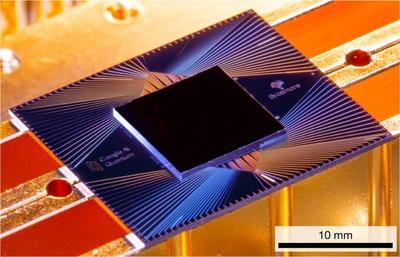
\includegraphics[width=0.7\linewidth]{1.jpeg}}
\caption{54-кубітний процесор Sycamore}
  
\end{figure}

У кожній точці надпровідної електронної схеми (тобто мережі електричних елементів) хвильова функція конденсату, що описує потік заряду, добре визначається конкретною комплексною амплітудою ймовірності. У звичайному електричному ланцюзі провідника такий самий квантовий опис справедливий для окремих носіїв заряду, проте різні хвильові функції усереднюються в макроскопічному аналізі, що унеможливлює спостереження за квантовими ефектами. Хвильова функція конденсату дозволяє проектувати та вимірювати макроскопічні квантові ефекти. Наприклад, лише дискретна кількість квантів магнітного потоку проникає через надпровідну петлю, подібно до дискретних рівнів атомної енергії в моделі Бора. В обох випадках квантування є результатом комплексної безперервності амплітуди. На відміну від мікроскопічних квантових систем (таких як атоми або фотони), що використовуються для реалізацій квантових комп’ютерів, параметри надпровідних ланцюгів можуть бути розроблені шляхом встановлення (класичних) значень електричних елементів, які їх складають, наприклад. регулювання ємності або індуктивності.\\ 

%Для того, щоб отримати квантовомеханічний опис електричного кола, необхідно виконати кілька кроків. По-перше, всі електричні елементи описуються амплітудою і фазою хвильової функції конденсату, а не тісно пов'язаним макроскопічним описом струму та напруги, що використовується для класичних схем. Наприклад, квадрат амплітуди хвильової функції в якійсь точці простору є ймовірністю знайти там носій заряду, отже, квадрат амплітуди відповідає класичному розподілу заряду. По-друге, узагальнені закони ланцюга Кірхгофа застосовуються до кожного вузла ланцюгової мережі для отримання рівнянь руху. Нарешті, рівняння руху переформульовано до лагранжової механіки і виведено квантовий гамільтоніан.

%%%%%%%%%%%%%%%%%%%%%%%%%%%%%%%%%%%%%%%%%%%%%%
\chapter{Надпровідні кубіти}\par 
Надпровідні кубіти реалізуються шляхом поміщення струму без опору в стан суперпозиції за допомогою мікрохвильового сигналу, коли він коливається навколо петлі ланцюга. Ця реалізація кубіта є найпоширенішою та є основною метою універсальних квантових комп’ютерів IBM і Google (серед інших).
\begin{figure}[h!]
\center{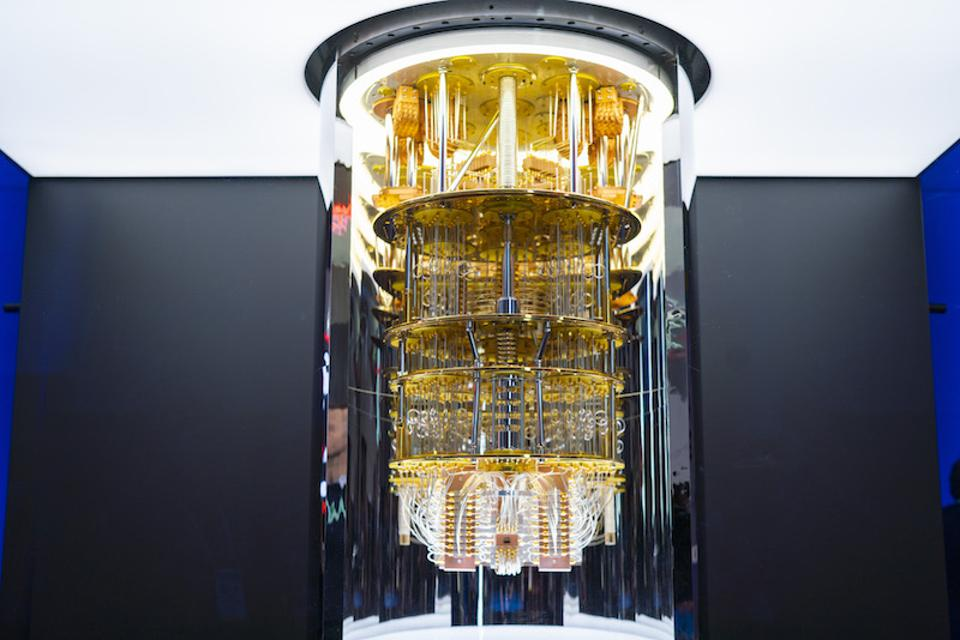
\includegraphics[width=0.9\linewidth]{3.png}}
\caption{Вигляд квантового комп'ютера на надпровідних кубітах}
\end{figure}
Сам надпровідний квантовий комп'ютер — це така бочка, що стоїть на ніжках, навколо якої знаходяться шафки з приладами, від приладів тягнуться пучки проводів, а за стінкою поруч, щоб менше шумів, тріщить вакуумний насос, який працює компресором у цьому холодильнику. Коли комп'ютер працює, він охолоджений до низької температури. Усередині бочки є диски, які розташовані один над одним. Верхній має температуру кілька градусів Кельвіна вище за абсолютного нуля, наступний — вже близько 1 градуса, і що нижча, то температура менша. Найнижча температура у нижнього диска, близько 0,02 K, зовсім поблизу абсолютного нуля, там знаходяться надпровідні кубити. Алюміній стає надпровідником вже при температурі близько 1 градуса вище абсолютного нуля, але потрібні стани |0$\rangle$ і |1$\rangle$ для коливань напруги в кубіті мають дуже маленьку різницю енергій $hv$, що відповідає мікрохвильовому випромінюванню.

\section{Переваги}
Надпровідні кубіти мають швидкий час роботи (обробки), що означає, що подібні обчислення можна виконувати набагато швидше, ніж на інших кубітах (наприклад, іонна пастка). Це важливо, оскільки корисні квантові обчислення, ймовірно, матимуть мільйони логічних елементів (операцій). Крім того, технологія, що лежить в основі надпровідних кубітів, може використовувати переваги існуючих методів і процесів (наприклад, друкованих схем), які ми вже витратили на вдосконалення десятиліттями. В результаті легше уявити масштабований надпровідний квантовий комп’ютер, ніж з деякими іншими існуючими методами.
\section{Недоліки}
Надпровідні кубіти мають швидкий час декогерентності, а це означає, що їхня «пам’ять» дуже короткочасна, і нам потрібно більше кубітів для виправлення помилок, щоб компенсувати. Оскільки надпровідні кубіти зазвичай можуть взаємодіяти лише з кількома кубітами поруч із ними на пристрої, нам потрібні додаткові операції для виконання більшості алгоритмів. Вони також повинні бути дуже холодними (нижче 100 мК або 0,1 градуса вище абсолютного нуля), що може бути дорогим і незручним. Нарешті, кожен надпровідний кубіт дещо відрізняється і повинен бути відкалібрований, що може викликати проблеми у великих системах.
%%%%%%%%%%%%%%%%%%%%%%%%%%%%%%%%%%%%%%%%%%%%%%
\chapter{Іонна пастка}\par 
Квантові комп’ютери з іонною пасткою працюють, захоплюючи іони (заряджені атоми) за допомогою електричних полів і утримуючи їх на місці, а самий зовнішній електрон, що обертається навколо ядра, може бути переведений у різні стани та використаний як кубіт.
\begin{figure}[h!]
\center{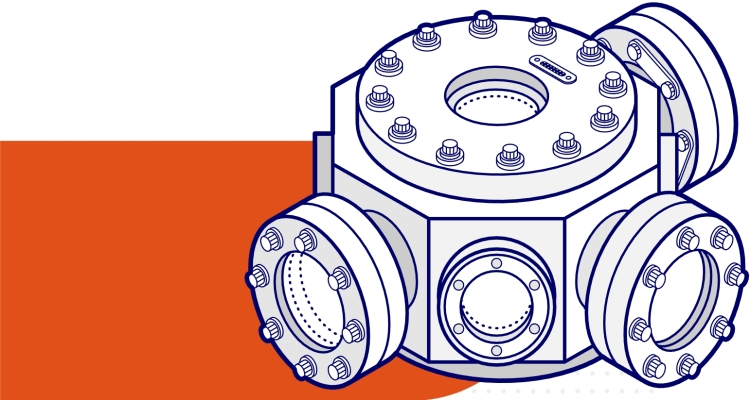
\includegraphics[width=0.7\linewidth]{2.jpg}}
\caption{Вакуумні камери, де динамічно розгортають та фіксують атомні кубити на кремнієвому чіпі, використовуючи електромагнітне поле}

\end{figure}

В іонних пастках використовуються іонізовані молекули з відповідною валентною структурою як регістри кубіту. Наразі компанія IonQ використовує іони Yb+ (ітербія). Іони - ідентичні і передбачувані у своїй поведінці - зручні у використанні. Зовнішні електрони можуть бути легко накачані до вищого енергетичного рівня і залишатися в цьому стані досить довго за мірками квантового світу. Залежно від свого стану молекула є нуль, одиницю або щось середнє. Подібні іони легко генерувати, вставляти в іонну пастку та утримувати їх там у стійкому стані. Взаємодія з ними здійснюється за допомогою зовнішніх лазерів, що переводять атоми в заданий стан. На відміну від надпровідних квантових комп'ютерів на основі напівпровідників, які, крім усього іншого, потребують спеціальних систем охолодження, системи з іонними пастками дешевші, їх легше створювати та експлуатувати.\\

\section{Переваги}
Головною особливістю комп’ютерів з технологією Ion Trap є їх стабільність; кубіти мають набагато довший «час когерентності», ніж ті, що використовуються в надпровідних квантових комп’ютерах. Хоча комп’ютер із іонною пасткою може працювати при кімнатній температурі, для досягнення найкращої продуктивності іони потрібно охолоджувати, але не в тій мірі, в якій це вимагає надпровідний квантовий комп’ютер. Зв’язки між кубітами іонної пастки можна переналаштувати, тобто кожен кубіт може взаємодіяти один з одним кубітом у комп’ютері, уникаючи деяких обчислювальних витрат, які виникають із надпровідними мікросхемами.
\section{Недоліки}
Комп’ютери з іонною пасткою, як правило, значно повільніші, ніж їхні надпровідні аналоги. Хоча їх не потрібно тримати холодними, іони мають бути у високому вакуумі. Технологія створення іонних пасток не настільки зріла, як у надпровідних кубітів, нам потрібно буде побачити значні покращення в цій області, перш ніж ми зможемо уявити масштабовану систему. Побудова квантового комп’ютера «Іонна пастка» вимагає інтеграції технологій з широкого діапазону областей, включаючи вакуумні, лазерні та оптичні системи, радіочастотну та мікрохвильову технологію, а також когерентні електронні контролери.




%%%%%%%%%%%%%%%%%%%%%%%%%%%%%%%%%%%%%%%%%%%%%%
\chapter{Нейтральні атоми}\par 
Нейтральні атоми – це подібний підхід до іонних пасток, але замість використання іонізованих атомів і використання їх заряду для утримання кубітів на місці використовуються нейтральні атоми та лазерний пінцет.
\section{Переваги}
Нейтральні атоми мають такий самий тривалий час когерентності, що й іони (використовуються в квантових комп’ютерах із іонною паскою). Його унікальною особливістю в порівнянні з іонними пастками є його потенціал для створення багатовимірних масивів. Ви можете прочитати більше в нашому ексклюзивному інтерв’ю з генеральним директором Atom Computing.
\section{Недоліки}
Масштабування системи нейтральних атомів стикається з проблемами, які виникають під час масштабування комп’ютера з захопленими іонами. Цей підхід продовжує розвиватися.
%%%%%%%%%%%%%%%%%%%%%%%%%%%%%%%%%%%%%%%%%%%%%%
\chapter{Топологічні кубіти}\par 

 Топологічні кубіти працюють за принципом, відмінним від інших кубітів, про які було сказано вище. Топологічні квантові обчислення намагаються реалізувати більш стійкий кубіт, використовуючи неабелеві форми матерії для зберігання квантової інформації. Неабелевими формами матерії є квазічастинки, як-от майорани ферміони та аньйони (неабелеві квазічастинки, які не є ні бозонами, ні ферміонами). Найперспективніші розробки топологічних квантових обчислень походять від неабелевого плетіння кіральних майоранівських ферміонів за допомогою квантових точок. Тип аніону, необхідний для створення універсального квантового комп’ютера, ще не підтверджений експериментально (але ми маємо деякі попередні ознаки). Поки що ця модель квантових обчислень є чисто теоретичною, але Microsoft досліджує топологічні кубіти протягом протягом кількох років. Топологічні кубіти повинні демонструвати високі часи когерентності та набагато вищу точність (менше помилок), ніж інші реалізації.\\ 

 Як вже згпдувалось раныше топологічні кубити більш стабільні, тому щоб усунути проблеми, пов'язані з крихкістю кубитів, Майкрософт використовує топологічні кубити, які стабілізуються за рахунок маніпулювання їхньою структурою та оточення їх хімічними сполуками, що захищають кубити від зовнішнього забруднення. Топологічні кубити захищені від шуму завдяки топологічним властивостям квазічастинок, що підвищує стійкість квантового обладнання Майкрософт до помилок. Ця підвищена стабільність дозволяє квантовому комп'ютеру масштабуватись, щоб виконувати більш тривалі та складні обчислення, а також спростити реалізацію більш комплексних рішень.
%%%%%%%%%%%%%%%%%%%%%%%%%%%%%%%%%%%%%%%%%%%%%%
\chapter{Висновок}
Основна проблема, що стоїть на шляху розробки квантових комп'ютерів, - це втрата кубіт когерентності. Будь-яка квантова система неминуче взаємодіятиме з оточенням, внаслідок чого відбуваються неконтрольовані зміни станів кубитів. Внаслідок цього серйозно підвищується ймовірність виникнення помилок у розрахунках. Крім того, низька когерентність кубіту загалом сильно обмежує кількість операцій, які може здійснити квантовий комп'ютер.\\

Це ключове обмеження кубітів вчені намагаються вирішити за допомогою створення «складних» логічних кубітів, які будуть складатися з кількох фізичних. Якщо кілька із них втратить когерентність, то решта все одно продовжить виконання завдання. Якщо такі складні системи вдасться отримати, тоді в міру розвитку технологій з'явиться шанс отримати безпомилкові квантові комп'ютери, здатні на необмежену кількість операцій.\\ 
 
Завдяки тому, що кубіти знаходяться в суперпозиції, квантові комп'ютери можуть набагато швидше виконувати деякі завдання за рахунок паралельного виконання декількох операцій. Наочний приклад користі від розпаралелювання - пошук шляху в лабіринті. Звичайний комп'ютер послідовно перебирає всі можливі варіанти, упираючись у глухий кут і повертаючись, а квантовий комп'ютер може перевірити всі можливі ходи за один раз.\\ 

Ефективність квантових комп'ютерів у вирішенні завдань такого типу настільки велика, що отримала назву квантової переваги. Для вирішення певних завдань по перебору квантового комп'ютера може знадобитися кілька хвилин, тоді як найпотужнішому класичному суперкомп'ютеру більше року. Найбільш корисною ця перевага може виявитися для моделювання хімічних та фізичних властивостей частинок, оптимізації побудови складних графів, створення більш продвинутих способів шифрування та дешифрування.\\ 

\begin{thebibliography}{9}
\bibitem{lit1} https://postnauka.ru/wtf/156211
\bibitem{lit2} https://azure.microsoft.com/ru-ru/overview/what-is-a-qubit/
\bibitem{lit3} https://habr.com/ru/post/480480/
\bibitem{lit4} https://en.wikipedia.org/wiki/Qubit
\bibitem{lit5} https://journals.aps.org/pra/abstract/10.1103/PhysRevA.100.062317
\bibitem{lit6} M. A. Nielsen and I. L. Chuang, Quantum Computation and Quantum Information(Cambridge, 2000).
\bibitem{lit7} https://link.springer.com/article/10.1007/s11128-004-3101-5

\end{thebibliography}

\end{document}